\section{Approach}
\label{sec:approach}
\begin{figure}[t]
\centering
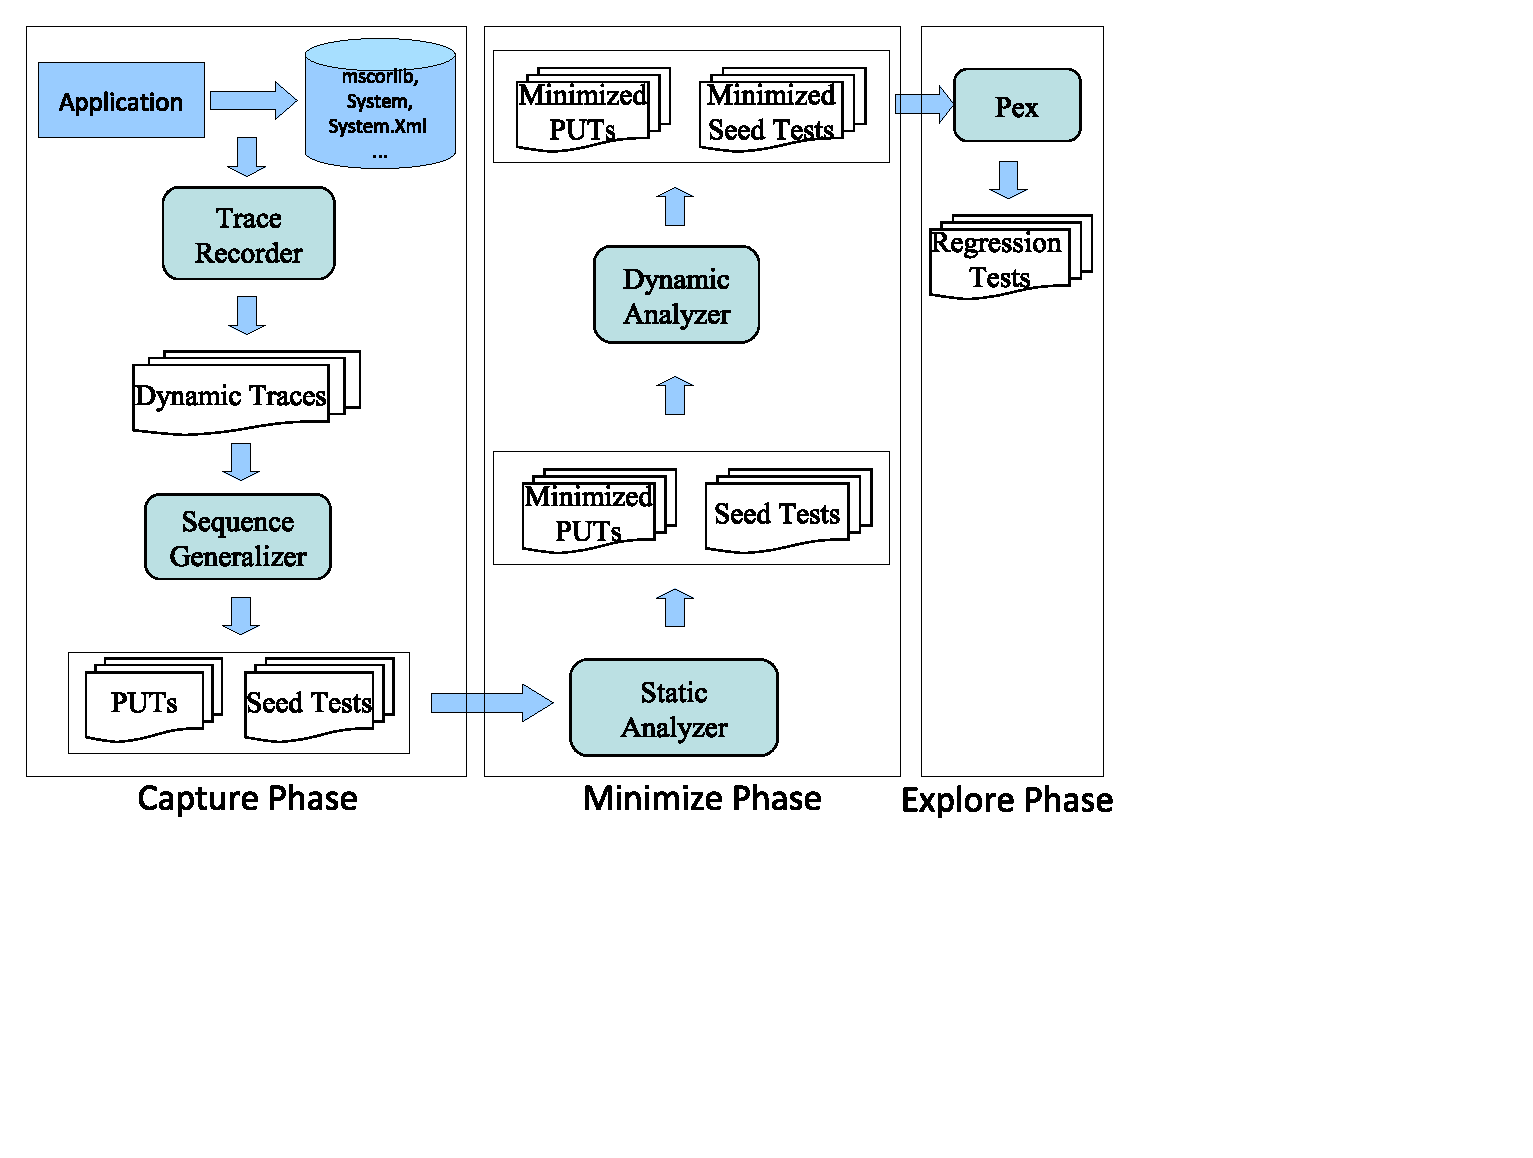
\includegraphics[scale=1,clip]{figure/approach.eps}\vspace*{-3ex}
 \caption{Overview of TeMaAPI}\vspace*{-4ex}
 \label{fig:approach}
\end{figure}
Given a migration tool between Java and C\#, TeMaAPI generates various test cases to reveal different behaviors of the tool's API mapping relations.
Figure~\ref{fig:approach} shows the overview of TeMaAPI.


%-------------------------------------------------------------------
\subsection{Generating client code}
\label{sec:approach:generating}
Given a migration tool, TeMaAPI first extracts its validate mapping relations of APIs. It is challenging to extract such mapping relations directly from a migration tool for two factors: (1) different migration tools may follow different styles to describe API mapping relations. For example, as shown in Section~\ref{sec:introduction}, the API mapping relations of Java2CSharp are described in its mapping files, but the API mapping relations of sharpen are hard-coded in its source files. (2) commercial migration tools typically hide their API mapping relations in binary files. Due to the two factors, TeMaAPI does not extract API mapping relations directly from a migration tool, but chooses to analyze translated code of a migration tool. If we use a migration tool to translate existing projects, many API mapping relations may be not covered, and it may be difficult to analyze the translated code for validate mapping relations. For the preceding consideration, TeMaAPI chooses to generate client code instead of using existing client code.

TeMaAPI relies on the reflection technique~\cite{maes1987concepts} provided by both Java and C\# to generate client code for translation. 

\textbf{Static fields.} Given a public static field \CodeIn{f} of a class \CodeIn{C} whose type is \CodeIn{T}, TeMaAPI generates a getter as follows:
\begin{CodeOut}%\vspace*{-2ex}
\begin{alltt}
 public T TestGet|f.name||no|()\{ return C.f; \}
\end{alltt}
\end{CodeOut}

If \CodeIn{f} is not a constant, TeMaAPI generates a setter as follows:
\begin{CodeOut}%\vspace*{-2ex}
\begin{alltt}
 public void TestSet|f.name||no|(T v)\{ C.f = v; \}
\end{alltt}
\end{CodeOut}

\textbf{Non-static fields.} Given a public non-static field \CodeIn{f} of a class \CodeIn{C} whose type is \CodeIn{T}, TeMaAPI generates a getter for each constructor \CodeIn{C(T1\ p1,\ldots, Tn\ pn)} of \CodeIn{C} as follows:
\begin{CodeOut}%\vspace*{-2ex}
\begin{alltt}
 public T TestGet|f.name||no|(T1\ c1,\ldots, Tn\ cn)\{ 
    C obj = new C(c1,\ldots, cn);
    return obj.f; \}
\end{alltt}
\end{CodeOut}

If \CodeIn{f} is not a constant, TeMaAPI generates a setter as follows:
\begin{CodeOut}%\vspace*{-2ex}
\begin{alltt}
 public void TestSet|f.name||no|(T1\ c1,\ldots, Tn\ cn)\{ 
   C obj = new C(c1,\ldots, cn);
   obj.f = v; \}
\end{alltt}
\end{CodeOut}

In the preceding code, ``\CodeIn{|f.name|}'' denotes the name of \CodeIn{f}, and ``\CodeIn{|no|}'' denotes the corresponding number of generated client-code method.

\textbf{Static methods.} Given a public static method \CodeIn{m(T1\ p1,\ldots,Tn\ pn)} of a class \CodeIn{C} whose return type is \CodeIn{Tm}, TeMaAPI generates a client-code method as follows:
\begin{CodeOut}%\vspace*{-2ex}
\begin{alltt}
 public Tm Test|m.name||no|(T1\ m1,\ldots, Tn\ mn)\{ 
   return C.m(m1,\ldots, mn); \}
\end{alltt}
\end{CodeOut}

\textbf{Non-static methods.} Given a public non-static method \CodeIn{m(T1\ p1,\ldots,Tn\ pn)} of a class \CodeIn{C} whose return type is \CodeIn{Tm}, TeMaAPI generates a client-code method for each constructor \CodeIn{C(Tv\ pv,\ldots, Tt\ pt)} of \CodeIn{C} as follows:
\begin{CodeOut}%\vspace*{-2ex}
\begin{alltt}
 public Tm Test|m.name||no|(T1\ m1,\ldots, Tn\ mn, 
                            Tv cv, \ldots, Tt ct)\{
   C obj = new C(cv,\ldots, ct);                     
   return obj.m(m1,\ldots, mn); \}
\end{alltt}
\end{CodeOut}

In the preceding code, ``\CodeIn{|m.name|}'' denotes the name of \CodeIn{m(T1\ p1,\ldots,Tn\ pn)}. 

TeMaAPI ignores generic methods for simplicity, and organizes all generated client code methods by the corresponding class $C$. For a migration tool that translates from Java to C\#, TeMaAPI generates client code in Java as shown by the solid line of Figure~\ref{fig:approach}, and for a migration tool that translates from C\# to Java, TeMaAPI generates client code in C\# as shown by the dotted line of Figure~\ref{fig:approach}. When TeMaAPI generates client code in C\#, it ignores \CodeIn{unsafe} and \CodeIn{delegate} methods and methods whose parameters are marked as \CodeIn{our} or \CodeIn{ref}. Java does not have corresponding keywords, so there are typically no mapped methods in Java for these C\# methods. After TeMaAPI generate client-code methods, we translate them using a migration tool under experiments.


%-----------------------------------------------------------------
\subsection{Analyzing Generated Methods}
\label{sec:approach:analyzing}
Translated code typically contain many compilation errors since a migration tool typically cannot cover mapping relations of all APIs. TeMaAPI then analyzes translated code for validate API mapping relations of the migration tool. To achieve this, TeMaAPI first remove all translated methods with compilation errors. For translated methods in Java, TeMaAPI implements a Eclipse plug-in that uses on Eclipse JDT compiler\footnote{\url{http://www.eclipse.org/jdt/}} for the list of compilation errors. For translated methods in C\#, TeMaAPI implements a Visual Studio.Net add-in to retrieve the list of compilation errors from the error-list view of Visual Studio.Net. Both Eclipse JDT compiler and Visual Studio.Net cannot list all methods with compilation errors in a single build. After each iteration of removing methods, TeMaAPI re-build these methods until it removes all methods with compilation errors.

After methods with compilation errors are removed, TeMaAPI compares generated code with translated code for the validate API mapping relations of a migration tool. Based on translated code and validate API mapping, TeMaAPI removes generated methods whose corresponding translated methods have compilation errors. We refer to those removing client-code methods as safe methods.

%-----------------------------------------------------------
\subsection{Generating and Executing Testing Cases}
\label{sec:approach:mappingmethods}
In the final step, TeMaAPI generates test cases to detect different behaviors of API mapping relations. For each safe method in Java, we use Randoop~\cite{pacheco2007feedback} to generate its test cases. For each safe method in C\#, we use Pex~\cite{tillmann2008pex} to generate its test cases. TeMaAPI then executes generated test cases, and records the inputs, the output, and the thrown exception of each test case as a file.

Based on the file, TeMaAPI generates Junit\footnote{\url{http://www.junit.org/}} or Nunit\footnote{\url{http://www.nunit.org/}} test cases to ensure each mapped API produce the same output give the same inputs. For example, Pex generates a test case whose input is \CodeIn{m0 = false} for the \CodeIn{TestvalueOf57} method in C\# as shown in Section~\ref{sec:example}, and after executing the output of the test case is ``False''. Based on the input and the output of this test case, TeMaAPI generates a Junit test case as follows:

\begin{CodeOut}%\vspace*{-2ex}
\begin{alltt}
 @Test
 public void testvalueOf64zhh0()\{
   sketch.Test_java_lang_String obj =
                       new sketch.Test_java_lang_String();
   boolean m0 = false;
   Assert.assertEquals("False", obj.testvalueOf64(m0));\}
\end{alltt}
\end{CodeOut}

This Junit test case fails since the preceding \CodeIn{testvalueOf64zhh} method produces ``false'' instead of ``False''. From this failed Junit test case, TeMaAPI detects that the \CodeIn{java.lang.String.valueOf (Object)} method in Java has different behaviors with its mapped C\# methods if inputs are boolean values.

In some cases, executing a test case does not produce outputs but exceptions. For example, Pex also generates a test case whose input is \CodeIn{m0 = null} for the \CodeIn{TestvalueOf57} method in C\# as shown in Section~\ref{sec:example}, after executing it throws \CodeIn{NullReferenceException}. TeMaAPI finds that the \CodeIn{NullPointerException} class in C\# is mapped to the \CodeIn{NullPointerException} class in Java in the validate API mapping relations, and generates a Junit test case based on the preceding mapping relation and input as follows:

\begin{CodeOut}%\vspace*{-2ex}
\begin{alltt}
 @Test
 public void testvalueOf64zhh3()\{
   try\{
     sketch.Test_java_lang_String obj =
                       new sketch.Test_java_lang_String();
     boolean m0 = null;
     obj.testvalueOf64(m0);\}
   \}catch(java.lang.NullPointerException e)\{
       Assert.assertTrue(true);
       return;
   \}
   Assert.assertTrue(false);\}
\end{alltt}
\end{CodeOut}

This Junit test case also fails since given a null input, the preceding \CodeIn{testvalueOf64} method does not throw any exceptions. From this failed Junit test case, TeMaAPI detects that the \CodeIn{java.lang. String.valueOf(Object)} method in Java has different behaviors with its mapped C\# methods if inputs are null pointers.

Each generated client-code method uses only one fields or methods provided by API libraries, and may lose some complicated behaviors even if test cases satisfy the round-trip criterion. To test those complicated behaviors, we introduce Java Compatibility Kit (JCK)\footnote{\url{https://jck.dev.java.net/}} that covers many complicated behaviors of Java APIs. JCK is a test suite provided by Sun to ensure compatibility of Java platforms, and it covers all APIs of J2SE. As JCK is released under read-only source license\footnote{\url{http://tinyurl.com/33x9fo6}}, we cannot generates Nunit test cases based on inputs and outputs by executing JCK. Instead, TeMaAPI reads source files of JCK, and translates API related test cases into Junit. For example, a test method for \CodeIn{java.lang.Strng.endWith (String)} in JCK is as follows:

\begin{CodeOut}%\vspace*{-2ex}
\begin{alltt}
  public Status String0044()\{
    String testCaseID = "String0044";
    String s1 = "endsWith Test"; //step Create a String
    String s2 = " Test";         //step Create a suffix
    ref.println("s1 = " + s1);
    ref.println("s2 = " + s2);
    if( s1.endsWith(s2) )        //step check result
    \{
       return Status.passed( "OKAY" );
    \}
       return Status.failed( testCaseID 
                             + " copyValueOf failed" );
    \}\}
\end{alltt}
\end{CodeOut}


Based on the test method of JCK, TeMaAPI generates a Junit method case as follows:

\begin{CodeOut}%\vspace*{-2ex}
\begin{alltt}
  @Test
  public void String0044()\{
    String testCaseID = "String0044";
    String s1 = "endsWith Test"; //step Create a String
    String s2 = " Test";         //step Create a suffix
    System.out.println("s1 = " + s1);
    System.out.println("s2 = " + s2);
    if( s1.endsWith(s2) )        //step check result
    \{
        Assert.assertTrue(true);
        return;
    \}
       Assert.fail();
       return;
    \}\}
\end{alltt}
\end{CodeOut}

JCK implements its own classes to assert whether a test case passes. To translate the preceding method of JCK into a Junit method, TeMaAPI follows the following steps:
 
\textbf{Step 1:} adding the \CodeIn{@Test} annotation to the method.

\textbf{Step 2:} the return type of the method \CodeIn{Status} $\rightarrow$ \CodeIn{void}.
 
\textbf{Step 3:} \CodeIn{return Status.passed(...)}  $\rightarrow$ \CodeIn{Assert.assertTure (true); return;} and \CodeIn{return Status.failed(...)} $\rightarrow$ \CodeIn{Assert. fail(); return;}. 

Some test methods of JCK are so straightforward as the previous one. For example, one test method for \CodeIn{java.io.File.delete()} in JCK is as follows:

\begin{CodeOut}%\vspace*{-2ex}
\begin{alltt}
  public Status File0037()\{
    String testCaseID = "File0037";
    ...
    FileRT method = new FileRT(testCaseID) \{
     public Status run() \{
       File f = null;
       f = new File(workdir, testCaseID); 
       ...
       if (f.delete()) \{ // Try to delete
         if (!f.exists()) \{ // Does it exist? 
           return Status.passed("OKAY");
         \}else\{
            return Status.failed(...);
         \}
       else\{
           return Status.failed(...);
       \}  
    \}
     return AllPermissionSM.testRun(...);
  \}
\end{alltt}
\end{CodeOut}

After the preceding three steps, TeMaAPI further replaces the statement starts with \CodeIn{FileRT} with the body of the \CodeIn{run} method, and removes the last statement. The translated code is as follows:

\begin{CodeOut}%\vspace*{-2ex}
\begin{alltt}
  public void File0037()\{
    String testCaseID = "File0037";
    ...   
    File f = null;
    f = new File(workdir, testCaseID);
    ...
    if (f.delete()) \{ // Try to delete
      if (!f.exists()) \{ // Does it exist?
        Assert.assertTrue(true);
        return;
     \}else\{
        Assert.fail();
        return;
     \}
   else\{
       Assert.fail();
       return;
   \}   
  \}
\end{alltt}
\end{CodeOut}

Compared with the original test method in JCK, the translated method does not use the \CodeIn{FileRT} class and the \CodeIn{AllPermissionSM} class. After the preceding process, TeMaAPI removes those test methods who use APIs out of the validate API mapping relations. As the \CodeIn{FileRT} class and \CodeIn{AllPermissionSM} class are both defined in JCK, their mapping relations are unlikely in the validate API mapping relations. Removing them increases the chance to translate a Junit test case into a Nunit test case. The remaining test cases can be translate by a migration tool from Java to C\# since their used APIs are all in the validate mapping relations of the migration tool.